\selectlanguage{italian}%

\section{Soluzione}


\subsection{Schematici}

\begin{figure}[H]
	\centering
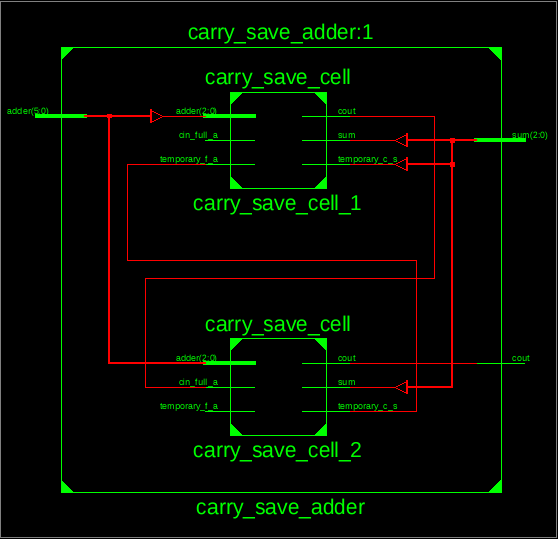
\includegraphics[scale=0.6]{esercizio10/images/carry_save_adder.png}
	\caption{Carry Save Adder}
\end{figure}Si � scelto di realizzare un semplice addizionatore di tipo carry
save che effettua la somma di due operandi da tre bit, nello schematico
sono mostrati due carry save cell, queste sono formate da due full
adder, uno utilizzato come carry save ed un altro come un full adder,
dopodich� i valori calcolari dal primo carry save cell vengono propagati
al secondo e la somma � determinata dalla uscita dei full adder.

\subsection{Codice}

\href{run:progetti/CarrySaveAdder/CarrySaveAdder.xise}{Carry Save Adder ISE}


\subsubsection{Carry Save Cell}

\lstinputlisting [language=VHDL,caption={Definizione della carry save cell},firstline=32] {progetti/CarrySaveAdder/carry_save_cell.vhd}

Come � realizzata una cella carry save citata sopra.\selectlanguage{italian}%

